\documentclass[review,number,sort&compress]{elsarticle}
\usepackage{lineno}


%\documentclass[preprint,12pt]{elsarticle}
\usepackage{amssymb}
\usepackage{lineno,hyperref}
\usepackage{subcaption}
\usepackage{graphicx}
\usepackage{booktabs}
\usepackage{textcomp}
\usepackage{setspace}
\onehalfspacing
\usepackage{multicol}

\usepackage{graphicx}
\usepackage{booktabs}
\usepackage{amssymb,bm,mathrsfs,amscd}
\usepackage[tbtags]{amsmath}
\usepackage{lastpage}
\usepackage{CJK}
\usepackage{booktabs}  %  ???????
\usepackage{amsfonts}
\usepackage{float}
\usepackage{siunitx}
%\usepackage{authblk}
%\modulolinenumbers[5]
%\setcitestyle{square}
%\journal{Nuclear Instruments and Methods A}
\journal{NIM-A}


%%%%%%%%%%%%%%%%%%%%%%%
%% Elsevier bibliography styles
%%%%%%%%%%%%%%%%%%%%%%%
%% To change the style, put a % in front of the second line of the current style and
%% remove the % from the second line of the style you would like to use.
%%%%%%%%%%%%%%%%%%%%%%%

%% Numbered
%\bibliographystyle{model1-num-names}

%% Numbered without titles
%\bibliographystyle{model1a-num-names}

%% Harvard
%\bibliographystyle{model2-names.bst}\biboptions{authoryear}

%% Vancouver numbered
%\usepackage{numcompress}\bibliographystyle{model3-num-names}

%% Vancouver name/year
%\usepackage{numcompress}\bibliographystyle{model4-names}\biboptions{authoryear}

%% APA style
%\bibliographystyle{model5-names}\biboptions{authoryear}

%% AMA style
%\usepackage{numcompress}\bibliographystyle{model6-num-names}

%% `Elsevier LaTeX' style
\bibliographystyle{elsarticle-num}
%%%%%%%%%%%%%%%%%%%%%%%

\begin{document}

\begin{frontmatter}

\title{The background of the JUNO calibration system }

%% Group authors per affiliation:
\author{Feiyang\corref{cor1}\fnref{fn1}}
\author{Yue Meng \corref{cor2}}
\address{Shanghai Key Laboratory for Particle Physics and Cosmology, Institute of Nuclear and Particle Physics (INPAC) and School of Physics and Astronomy, Shanghai Jiao Tong University, Shanghai 200240, China}
\cortext[cor1]{Corresponding author}
\begin{abstract}
Jiangmen Underground Neutrino Observatory (JUNO) is reactor neutrino detector with 20 kton liquid sctitillator as a target. The main goal of JUNO is to determine the neutrino mass hierarchy (MH) via precisely measurement of anti-neutrino oscillation spectrum. The measurement requires high energy resolution (3\% at 1 MeV) and small uncertainty (less than 1\%), which give a huge challenge to calibration system. The devices of calibration system close to the central detector will increase the background, which worsen the energy resolution and thereby lower the MH sensitivity. In addiction, the background will also deteriorate other neutrino spectrum like supernova neutrino, solar neutrino and so on. In this study, we will discuss the contribution background from calibration system. 
\end{abstract}

\begin{keyword}
JUNO, Calibration, background, radioactivity.
\end{keyword}
\end{frontmatter}
\linenumbers
\section{The JUNO Introduction}
Jiangmen Underground Neutrino Observatory (JUNO) is a multi-purpose neutrino experiment. 
The main goal of JUNO is to determine the neutrino mass hierarchy (MH) via precisely measuring reactor anti-neutrino oscillation spectrum. 
%The experiment is located 700 m underground in Guangdong, China, with distance of 53 km from Yangjiang and Taishan nuclear power plant (NPP).

%However, the background from radioactive and cosmogenic isotopes will reduce the efficiency of neutrino events selection. 
%To reduce the background from cosmic rays (i.e. muon), the JUNO experiment is located in 700 m underground.
The JUNO experiment is in Jiangmen city, Guangdong province, China, 53 km from Yangjiang and Taishan nuclear power plants (NPP).
The target of JUNO is 20 kton liquid scintillator with 12 cm thickness spherical acrylic shell as container.
The central detector is a 35.4 m diameter ball within a water pool.
The water pool a 40 m hight and 40 m diameter cylinder filled with ultra-pure water as a buffer to stop the external radioactivity. 
There are about 18000 20-inch and 25000 3-inch photomultipliers (PMTs) closed the central detector with about 75\% coverage.

The reactor anti-neutrino could be detected via so-called inverse beta decay (IBD) reaction, $\bar{\nu}_{e}+p \rightarrow e^{+}+n $.The positron will deposit energy first as a prompt signal, while the neutron will be captured by the nuclear (proton or carbon) within about 200 us as a delay signal. 
With the pair of prompt signal positron and delay signal neutron, the efficiency of IBD events selection could be significantly improved. 
However, the background of physics-like events will smear the prompt and delay signal, which will reduce the efficiency and quality.
Two physics-like events from background with interval time of about 200 us will be falsely identified as IBD events.
And the extra introduced background events will distort the reactor neutrino spectrum, and thereby worse the neutrino MH sensitivity. 

The background is mainly from cosmogenic and nature radioactive isotopes.
In the LS, the interaction of energetic cosmic muons with C-12 will produce radioactive isotopes like Li-9, He-8, B-12 and so on.
The radioactive isotope is not stable and will decay to emit alpha, beta and gamma particles.
Especially for Li-9 and He-8, they can emit both a beta and a neutrino, just like a IBD signal, which will significantly influence the efficiency of IBD selection.  
The other background source, nature radioactive isotopes is from kinds of material used in the experiment.
The isotopes mainly include U-238, Th-232, and K-40, which have long-lived time at billion years level.
The radioactive material includes LS, acrylic, stainless steel, PMT and material from calibration system.
In principle, the closer to detector, the more significant of background contribution to experiment.
Since the part of calibration device is close and even in the central detector, so the background of calibration system contribution should be significantly treated. 

In this paper, we will study the influence of calibration system on the JUNO experiment background, which consists of the following ingredients: 
\noindent
Measurement of radioactive material of calibration system.
\noindent
Background contribution via MC simulation.
\noindent
The influence on MH sensitivity.

\section{The JUNO calibration system}

The JUNO calibration system is designed 
to mainly correct the energy response of non-linearity 
and detector non-uniformity, which requires the multiple 
sources to reach multiple locations.
To meet the calibration requirement, there is no choice to totally avoid contact with the central detector even some components permanently in it.
The calibration systems includes 4 deployment sub-systems as shown in Fig.~\ref{calib:systems} and 2 positioning sub-systems. 

\begin{figure}[h]
	\centering
	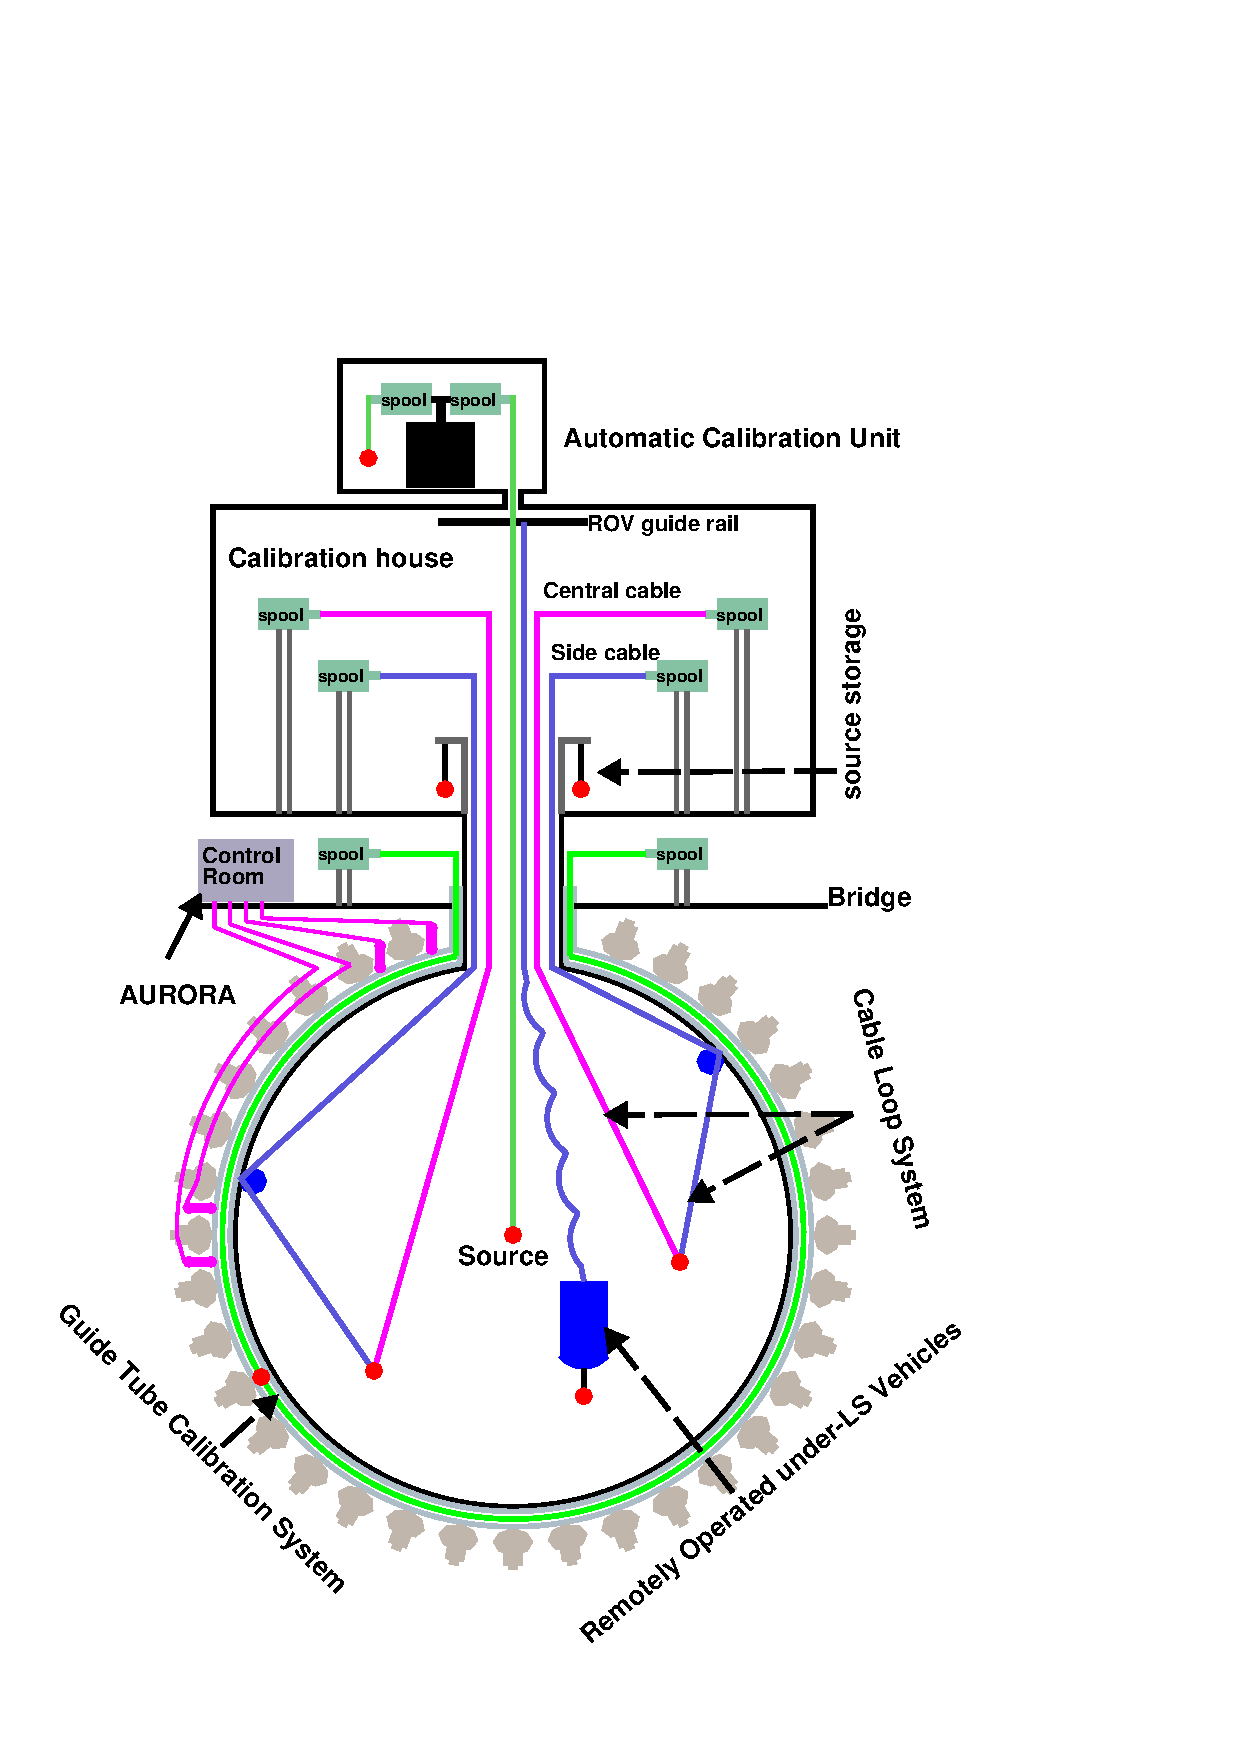
\includegraphics[width=3in]{calib_systems.pdf}
	\caption{The overview of JUNO Calibration systems}
	\label{calib:systems}
\end{figure}

\subsection{Automatic Calibration Unit (ACU)}

The ACU is located at the top of the calibration house, which keep away from the central detector (CD).
So normally, the contribution of ACU can be ignored.
Only in the calibration turn, the calibration source of ACU attached on cable will enter the CD.
The routine calibration sources include laser source and radioactive source. The rate of laser source and radioactive source are respectively 50 Hz and 100 Hz. The only fact we should concern is whether the background rate of cable is enough high to affect the calibration data.


\subsection{Cable Loop System (CLS)}
The strategy of CLS is to deploy the calibration sources offaxis position in half-plane.
There are two asymmetric CLSs designed as illustrated in Fig?.
For each CLS, central cable and side cable ware attached to the source formaing a loop to deliver and retract the source.
And the side cable will go through a anchor, a piece of 3.2 kg PTFE attached on inner surface of acrylic shell.
Based on the design of CLS, part of side cables will be permanently in the central detector (CD) during the physics data taking. The length of cable in the CD is ?? m, and the total mass is ?? kg.
The core of the cable is stainless steel (SS), while the shell is PTFE.

\subsection{Guide Tube Calibration System (GTCS)}
The GTCS is a tube looped outside of the acrylic sphere along a
latitude line, within which a radioactive source with cables attached
to both ends gets driven around with good positioning precision.  The
design of this system is discussed in details in
Ref.~\cite{GTCS}. MeV-scale gammas can easily penetrate the 12~cm acrylic
and deposit energy in the LS region, although the full absorption peak
is mixed with a somewhat significant leakage tail.
The PTFE tube, the cable and position sensor is close to the CD.
The background of their contribution is a non-negligible value and 
should be seriously studied.

\subsection{Remotely Operated under-LS Vehicles (ROV)}

ROV is designed to deploy the source in CD with a 3-D scanning.
The ROV is not a routine calibration system, the frequency of ROV calibration
is at one time per year level.
And usually the device is in the calibration house, which is far away from the CD.
So the background contribution of ROV can be negligible.

\subsection{USS}

USS is a significant component of JUNO calibration system. 
The system is permanently in JUNO central detector for calibration source position determination. 
To avoid the problem of multiple paths that will worse the precision of position measurement, 
the USS receiver will will be installed in the inner of CD, meaning that it will permanently contact with LS.
Since the components of USS are in the LS of JUNO, it will introduce non-negligible background to the detector. 

The radioactivity isotopes will emit MeV energy level particles (alpha, beta, gamma), which is in the energy range of physics events.
These particles will enter to the detector and be detected, resulting signal disturbing the real physics signal, which is called background. So controlling the background of USS is a work for JUNO calibration.
The USS includes cables, which is close the Acrylic inner sphere, with total length xx m, and 8 ultrasonic receivers, which is attached on acrylic shell. The USS cables consist of Teflon and stainless steel (SS), with diameter 1 mm. The line density is 0.01 kg/m. The ultrasonic receivers consist of two parts, NI and PCB with mass 0.106 kg. 

\subsection{CCD}

\subsection{AURORA}

\section{Radioactive background}
\subsection{Potential background}

The isotopes we should consider in background estimation include 
$^{238}U$, $^{232}Th$, $^{40}K$, $^{137}Cs$, Radon, and Kr.
Among them, $^{238}U$, $^{232}Th$ and $^{40}K$ are long-lived isotopes with billion years life time,
so the rate of decay is stable within 20 years running.
$^{238}U$ is one isotope of uranium in nature with a abundance of 99\%.
The life time of $^{238}U$ is about 4.47 $\times10^{9}$ years.
Besides $^{238}U$ decay, the daughter isotope is also not stable and will decay, 
which should be considered during the background calculation.
And a series of daughter isotopes construct a decay chain.
Beginning with naturally occurring $^{238}U$, 
And life time of the daughter isotope is pretty short compared with $^{238}U$.
So in the equilibrium state of decay, the rate of every daughter isotope should be equal to the rate of $^{238}U$ decay.
$^{232}Th$ is one isotope of thorium, with abundance almost 100\%, life time 1.4 $\times10^{10}$ years.
Just similar to $^{238}U$, $^{232}Th$ also has a decay chain.
$^{40}K$ is one of potassium isotopes with life time 1.25 $\times10^{9}$ years, abundance 0.012\%.
Different from $^{238}U$ and $^{232}Th$, $^{40}K$ doesn't have decay chain. 

Compared with $^{238}U$, $^{232}Th$ and $^{40}K$, 
the life time of $^{137}Cs$ ${60}Co$ is pretty short with only several or several tens of years. 
For most material, the rate of them is too low to test, but they also should be considered if the rate is very high.


The emission particles from decay include gamma, beta and alpha, which is isotopes dependent.

\noindent
1. isotopes: U,Th,K,Cs,Co, Radon, Kr. \\
2. decay: gamma, beta, alpha,\\
3. bulk: surface, emanation\\

\subsection{Requirements and budget}

The main background is from LS, 
The overall budget should be kept less than 0.2 Hz.

\begin{center}
	\centering
	\begin{tabular*}{150mm}{@{\extracolsep{\fill}}ccccccc}
		\toprule  % ???
               Calibration component location & Items\\
		\midrule  % ???
	       Inside CD (permanently) & USS receivers\\
               Inside CD (permanently) & USS cable\\
               Inside CD (permanently) & CLS cable\\
               Inside CD (permanently) & Anchor and mounting structure\\
               Inside CD (permanently) & Surface cleanliness\\
		\midrule  % ???
	       Radon emanation of the calibration house & ACU/CLS spool/ROV/Calibration house\\
		\midrule  % ???
		Outside CD (permanently) & GT\\
		Outside CD (permanently) & CCD \\
		Outside CD (permanently) & AURORA\\
		 \bottomrule  % ???
\end{tabular*}
\end{center}

\section{Simulation method, cut}
\subsection{Simulation method}
SNIPER is an official tool to simulate JUNO experiment. The main detector geometry is developed by JUNO software members, but not including USS related geometry. So first, we need draw the geometry of USS, and put it into the whole detector in correct position. And then assume the radioactive sources (U238, Th232, K40) are uniformly distributed in the material. The simulation will run for every component independently. After the simulation, the total PE spectrum will be obtain as shown in Fig.~\ref{USS:Rece:U238}.

\begin{figure}
	\centering
	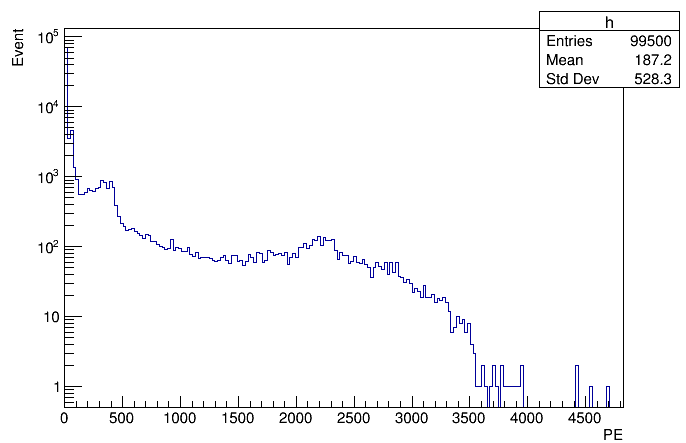
\includegraphics[width=3in]{U238_USS_receiver.png}
	\caption{Simulation for U238 in USS receiver}
	\label{USS:Rece:U238}
\end{figure}

\subsection{Energy and Fiducial volume cut}


With the MC simulation, we can calculate the efficiency of radioactivity particles detected.
However, the truth is that not all events can affect the real physics signal. 

Considering that the energy of prompt IBD signal is above 1 MeV.
So one energy cut of 700 keV could basically remove 
the low energy events that won't affect the IBD spectrum.

Duo to the sharply increased background, poor calibration and bad vertex reconstruction at the boundary of detector, 
the quality of physics events at the boundary will decrease.
To ensure the quality of physics events, 0.5 m cut will be carried out during calculation, which means that we only calculate the events with radius less than 17.2m (the radius of detector is 17.7m).

\subsection{Survival probability}

With given number of simulation events, after above cut, a ratio of residual events and the initial events can be calculated.
The ratio is called survival probability, which is radioactive isotopes, positions and geometry dependent. 
The survival probability is one of the key points to reflect the importance to the detector background.
And with known survival probability and material radioactivity, the background contribution to the detector could be calculated.

Table? shows the summary of survival probability of calibration system survival probability.


Analysis the results for each sub-systems ....

\section{Radioactivity measurement}
To control the background from JUNO calibration system, first we need to select pure material with low radioactivity. 
We used the high pure germanium detector located in Jinpin underground experiment to test the radioactivity of the material as shown in Fig 1.
The table 1 shows the testing result, which is best material we obtain so far. The Th232 and U238 radioactivity is measured from two daughter isotope, to be conservative, we use the maximum of the two value as the final material radioactivity. The result seems good with low radioactivity. But to preciously calculate the background contribution, we need MC simulation to scale the value.

\begin{figure}[h]
	\centering
	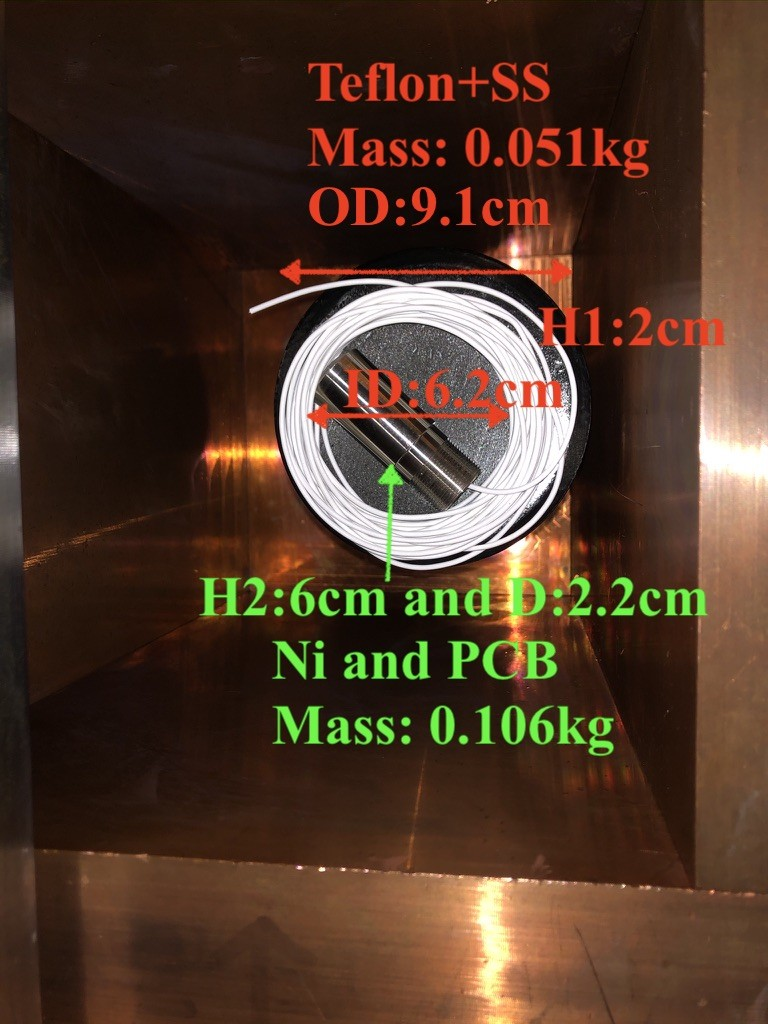
\includegraphics[width=3in]{USS_Cable_PCB_Ni.png}
	\caption{JUNO USS cables and receivers. They are in high pure germanium detector for radioactivity testing}
	\label{USS_Cable_PCB}
\end{figure}


\section{Radioactive background result}

\subsection{Calibration systems}

\subsubsection{ACU}

Since there are no component of ACU permanently in central detector, so the only concern about ACU background contribution is for calibration data.
The background is from mechanical cable for radioactive source and optical fiber for laser source.
The background rates of mechanical cable and optical fiber are respectively ?? mHz and ?? mHz, negligible compared with the calibration source. 

\subsubsection{CLS}

The mechanical cable of CLS and corresponding anchor will be permanently in CD. 
The contribution background of CLS is shown in Table ?.

The anchor is at the boundary of CD, contact with the acrylic inner surface, so with the fiducial volume cut, most of background event will be removed resulting low rate of contribution. 
However, based on the CLS design, most of mechanical cable is in the fiducial volume, so even with fiducial volume cut, it is still difficult to significantly decrease the background rate.

\begin{tabular*}{100mm}{@{\extracolsep{\fill}}ccccccc}
	\toprule  % ???
	Isotope	& Rate (mHz)&	Err (mHz)\\
	\midrule  % ???
	Co60	& 	0.056&	0.088	\\ 
	K40	& 	0.309&	0.226	\\
	Th232&	0.520&	0.214	\\
	U238 &    0.419&	0.143	\\
	Total (mHz)&	0.987&	0.574	\\
	\bottomrule  % ???
\end{tabular*}

\begin{tabular*}{100mm}{@{\extracolsep{\fill}}ccccccc}
	\toprule  % ???
	Isotope	&	Rate (mHz)&	Err (mHz)\\
	\midrule  % ???
	U238	&	0.162	  &      0.327\\ 
	Th232	&	2.470	  &      0.573\\
	K40	&	0.712	  &      0.424\\
	Total(mHz)&	3.344	  &      0.784\\
	\bottomrule  % ???
\end{tabular*}

\subsubsection{GT}


\begin{tabular*}{150mm}{@{\extracolsep{\fill}}ccccccc}
	\toprule  % ???
	Isotope	& Rate (mHz)&	Err (mHz)\\
	\midrule  % ???
	Co60	& 	0.056&	0.088	\\ 
	K40	& 	0.309&	0.226	\\
	Th232&	0.520&	0.214	\\
	U238 &    0.419&	0.143	\\
	Total (mHz)&	0.987&	0.574	\\
	\bottomrule  % ???
\end{tabular*}

\begin{tabular*}{150mm}{@{\extracolsep{\fill}}ccccccc}
	\toprule  % ???
	Isotope	&	Rate (mHz)&	Err (mHz)\\
	\midrule  % ???
	U238	&	0.162	  &      0.327\\ 
	Th232	&	2.470	  &      0.573\\
	K40	&	0.712	  &      0.424\\
	Total(mHz)&	3.344	  &      0.784\\
	\bottomrule  % ???
\end{tabular*}

\subsubsection{USS}
\begin{tabular*}{150mm}{@{\extracolsep{\fill}}ccccccc}
	Isotope	& Rate (mHz)&	Err (mHz)\\
	\toprule  % ???
			&   Rate(mHz)&	Err(mHz)&Err(mHz)\\
	\midrule  % ???                             
	Co60		& 	0.056&	0.088	&0.088	\\ 
	K40		& 	0.309&	0.226	&0.226	\\
	Th232		&	0.520&	0.214	&0.214	\\
	U238 		&    	0.419&	0.143	&0.143	\\
	Total (mHz)	&	0.987&	0.574	&0.574	\\
	\bottomrule  % ???
\end{tabular*}

\begin{tabular*}{150mm}{@{\extracolsep{\fill}}ccccccc}
	\toprule  % ???
	Isotope	&	Rate (mHz)&	Err (mHz)\\
	\midrule  % ???
	U238	&	0.162	  &      0.327\\ 
	Th232	&	2.470	  &      0.573\\
	K40	&	0.712	  &      0.424\\
	Total(mHz)&	3.344	  &      0.784\\
	\bottomrule  % ???
\end{tabular*}

\subsection{Influence to total JUNO background}

The total rate of background from calibration system is about ?? mHz, which meet the required budget.

\section{Conclusion}

With HGe detector, we have tested the radioactivity all the material from calibration system.
And with geant4-based detector simulation, we have calculated the rate of background with energy and fiducial volume cut.
The total rate is less than ?? mHz, which meets the requirement.
The degeneration of MH sensitivity due to calibration system background is about ??.

\section{Acknowledgement}
\section*{References}
\bibliography{mybibfile}
\end{document}
